
\documentclass[12pt]{article}

% Layout.
\usepackage[top=1in, bottom=0.75in, left=1in, right=1in, headheight=1in, headsep=6pt]{geometry}

% Fonts.
\usepackage{mathptmx}
\usepackage[scaled=0.86]{helvet}
\renewcommand{\emph}[1]{\textsf{\textbf{#1}}}

% TiKZ.
\usepackage{tikz, pgfplots}
\usetikzlibrary{calc}
\pgfplotsset{compat = newest}
 
\pgfplotsset{my style/.append style={axis x line=middle, axis y line=
middle, xlabel={$x$}, ylabel={$y$}, axis equal }}

% Misc packages.
\usepackage{amsmath,amssymb,latexsym}
\usepackage{graphicx}
\usepackage{array}
\usepackage{xcolor}
\usepackage{multicol}

% Commands to set various header/footer components.
\makeatletter
\def\doctitle#1{\gdef\@doctitle{#1}}
\doctitle{Use {\tt\textbackslash doctitle\{MY LABEL\}}.}
\def\docdate#1{\gdef\@docdate{#1}}
\docdate{Use {\tt\textbackslash docdate\{MY DATE\}}.}
\def\doccourse#1{\gdef\@doccourse{#1}}
\let\@doccourse\@empty
\def\docscoring#1{\gdef\@docscoring{#1}}
\let\@docscoring\@empty
\def\docversion#1{\gdef\@docversion{#1}}
\let\@docversion\@empty
\makeatother

% Headers and footers layout.
\makeatletter
\usepackage{fancyhdr}
\pagestyle{fancy}
\fancyhf{} % Clears all headers/footers.
\lhead{\baselineskip 30pt
%\emph{\@doctitle\hfill\@docdate}
\emph{\@docdate\hfill\@doctitle}
\ifnum \value{page} > 1\relax\else\\
\emph{Name: \rule{3.5in}{1pt}\hfill \@docscoring}\fi}
\rfoot{\emph{\@docversion}}
\lfoot{\emph{\@doccourse}}
\cfoot{\emph{\thepage}}
\renewcommand{\headrulewidth}{0pt}%
\makeatother

% Paragraph spacing
\parindent 0pt
\parskip 6pt plus 1pt

% A problem is a section-like command. Use \problem{5} to
% start a problem worth 5 points.
\newcounter{probcount}
\newcounter{subprobcount}
\setcounter{probcount}{0}
\newcommand{\problem}[1]{%
\par
\addvspace{4pt}%
\setcounter{subprobcount}{0}%
\stepcounter{probcount}%
\makebox[0pt][r]{\emph{\arabic{probcount}.}\hskip1ex}\emph{[#1 points]}\hskip1ex}
\newcommand{\thesubproblem}{\emph{\alph{subprobcount}.}}

% Subproblems are an enumerate-like environment with a consistent
% numbering scheme. 
% Use \begin{subproblems}\item...\item...\end{subproblems}
\newenvironment{subproblems}{%
\begin{enumerate}%
\setcounter{enumi}{\value{subprobcount}}%
\renewcommand{\theenumi}{\emph{\alph{enumi}}}}%
{\setcounter{subprobcount}{\value{enumi}}\end{enumerate}}

% Blanks for answers in normal and math mode.
\newcommand{\blank}[1]{\rule{#1}{0.75pt}}
\newcommand{\mblank}[1]{\underline{\hspace{#1}}}
\def\emptybox(#1,#2){\framebox{\parbox[c][#2]{#1}{\rule{0pt}{0pt}}}}

% Misc.
\renewcommand{\d}{\displaystyle}
\newcommand{\ds}{\displaystyle}
\def\bc{\begin{center}}
\def\ec{\end{center}}
\def\be{\begin{enumerate}}
\def\ee{\end{enumerate}}


\doctitle{Math 251: Quiz 9}
\docdate{November 4, 2021}
\doccourse{UAF Calculus I}
\docversion{v-1}
\docscoring{\blank{0.8in} / 25}
\begin{document}

There are 25 points possible on this quiz. No aids (book, calculator, etc.)
are permitted.  {\emph{Show all work for full credit.}}

\problem{9} (Optimization) You need to construct a rectangular fence that encloses an area of 300 square feet. The two vertical sides (drawn solid below) will be made of material that costs \$5 per foot while the material for the horizontal sides (drawn dashed below) costs \$2 per foot. Determine the dimensions of the least expensive fence. Make sure you explicitly address the items below.\\

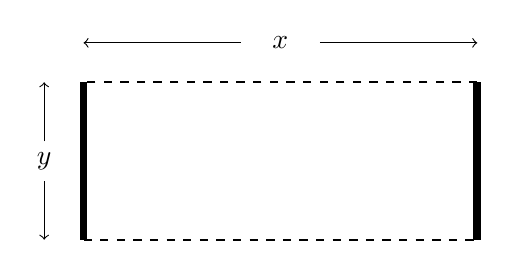
\begin{tikzpicture}
\draw[<-] (0,2.5) -- (2,2.5);
\draw[->] (3,2.5) -- (5,2.5);
\node at (2.5,2.5){$x$};
\draw[<-] (-.5,0) -- (-.5,.75);
\draw[->] (-.5,1.25) -- (-.5,2);
\node at (-.5,1){$y$};
\draw[line width=1mm] (0,0) -- (0,2) (5,0) -- (5,2);
\draw[thick, dashed] (0,0) -- (5,0) (5,2) -- (0,2);
\end{tikzpicture}
\begin{subproblems}
	\item Explicitly state the quantity you want to maximize or minimize.
	\item Identify the domain of your function.
	\item Identify your answer. (Note: Your answer may not be an integer.)
	\item Justify that your answer is correct. That is, use Calculus to show that your answer indeed does represent a maximum or minimum.
	\vspace{2in}
\end{subproblems}
\newpage
\problem{8} Evaluate the following limits. Before an application of L'H\^{o}pital's Rule, you must indicate the form of the limit ($0/0$ or $\infty/\infty$).
\begin{subproblems}
	\item $\ds \lim_{x \to 1} \frac{x^{14} -1}{x^5-1} $
	\vfill
	\item $\ds \lim_{x \to \infty} \left(1+\frac{2}{x}\right)^{x} $
	\vspace{3in}
\end{subproblems}
\problem{8} Evaluate the following indefinite integrals.
	\begin{subproblems}
	\item $\ds \int \left( 2 + x +\frac{1}{x^2} \right) \: dx$
	\vfill
	\item $\ds \int \left( \sec(x)\tan(x)+e^x \right) \: dx$
	\vfill
	\end{subproblems}
\end{document}